







\section{Experimental results}\label{05}
In this section we present all the obtained results of our experiments. First of all we report our attempts on tuning the system components: policy, annotator and reward model. We also explore different kind of Oracle that we exploit to train faster our system, since with only human annotations the training time would have been longer. Finally we underline the grown of reward model loss.




\subsection{Hyper-parameters Tuning}        % Setting IRL components
We implement an IRL system which include three principal components: a policy, an annotator and a reward model. Our aim is to force the agent to achieve the goal trough the left bottom corner of the map, for a total of 9 agent steps (one more step with respect to the optimal goal trajectory).

Each iteration the policy makes 150 episodes each one composed by 150 agent steps. The dimension of an episode is an important value, since, in order to converge, it's essential that the agent reaches the goal as often as possible in the first iterations of the training process. 


%%%%%%%%%%%%%%%%%%%%%%%%%%%%%%%%%%%%%%%%%%%%%%%%%%%%%%%%%%%%%%%%%%%%%%%%%%%%%%%%%%%%%%%%%%%%%%%
\begin{figure}[t]
    \centering
    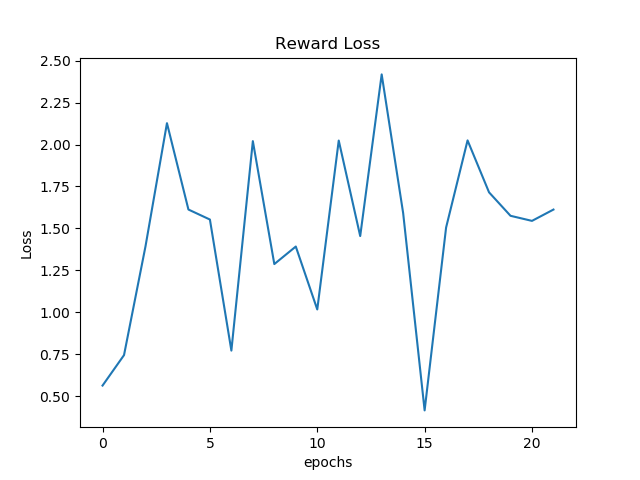
\includegraphics[width=\linewidth]{data/reward_loss.png} 
    \caption{Reward model loss with early stop after 25 iterations.}
	\label{fig:rewardloss}%
\end{figure}
%%%%%%%%%%%%%%%%%%%%%%%%%%%%%%%%%%%%%%%%%%%%%%%%%%%%%%%%%%%%%%%%%%%%%%%%%%%%%%%%%%%%%%%%%%%%%%%

In Inverse Reinforcement Learning the policy does not take rewards from the environment but from the reward model, that is trained to assign a reward $r\in R$ to each agent state. Since the reward model is trained only comparisons (like we described in section \ref{method}), we perform a standardization, with $0$ mean and $0.5$ of std, on the reward model output, because it's scale-free. The std value is empirical and it has a huge impact on the system's performance: larger values of it imply bigger rewards in every agent step, while smaller ones often result in negative goal reward. In the first iterations, the majority of clips show the agent in the upper part of the map trying to learn some environment rules. This involves that the reward model does not learn nothing about the bottom states, especially the goal state. So the agent learns different environment rules respect to the ones that we want to teach him.
When we set std to 1 or surrounding values, the agent learned to stand still, since the upper states provide him higher rewards. In the other scenario, when std is about 0.05 (like the authors of \cite{NIPS2018_8025} adopted in their work), rewards got a so small range of possible values that the agent receive a negative reward in the goal state. Thus we find that values between $0.5$ and $0.6$ are the best choices for std of agent rewards. 
The standardization is performed on the last 300 agent step rewards, two episodes approximately, that allow us to compute the right values' range comparing same agent action distributions.

%%%%%%%%%%%%%%%%%%%%%%%%%%%%%%%%%%%%%%%%%%%%%%%%%%%%%%%%%%%%%%%%%%%%%%%%%%%%%%%%%%%%%%%%%%%%%%%
\begin{figure}[t]
    \centering
    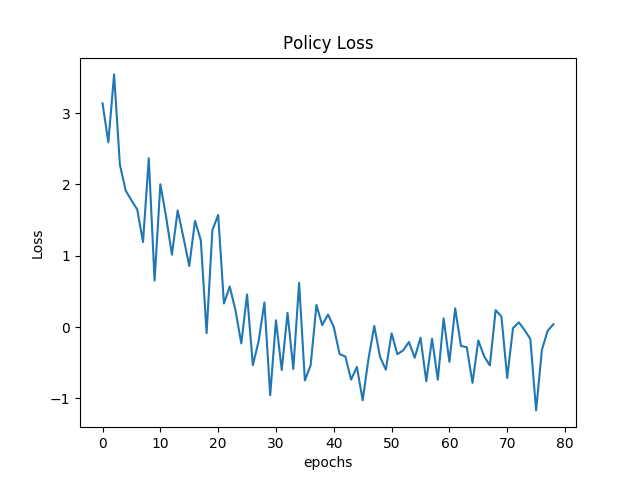
\includegraphics[width=\linewidth]{data/policy_loss_80.png} 
    \caption{Policy model loss after 80 training iterations.}
	\label{fig:losspolicy}%
\end{figure}
%%%%%%%%%%%%%%%%%%%%%%%%%%%%%%%%%%%%%%%%%%%%%%%%%%%%%%%%%%%%%%%%%%%%%%%%%%%%%%%%%%%%%%%%%%%%%%%

We set the clip length to 5. We choose that value because we want to force a trajectory of 9 agent steps. 
For this reason with length of 5, clips are big enough to show if the agent is computing movements in the trajectory we wanted to teach him, or not. The result is that the "perfect trajectory" is composed by two clips. The first where the agent turns down, runs across the left part of the map and, again, turns towards the goal. In the second the agent simply goes forward until its destination, that need just 4 moves. For this reason the corresponding clip will have the goal state replicated twice. 

Our experiments are carried out with an Oracle, that gives preferences regarding handcrafted rules. To define this, we have to generate a matrix that corresponds to the environment structure where each position has its reward. Our aim is that the reward model will learn this Oracle matrix from the annotations without ever seeing it. In particular, we explore different types of that artificial annotator, one where there are smoother values of matrix, and another matrix with sparse values. Both of them have reward 1 in each state of the trajectory that we want to force to the agent, and 10 as the goal reward. The difference between the two versions are in the rewards of the other states that are not in this trajectory. 
The sparse Oracle has 0 as reward for all these states, while the smooth Oracle sets those rewards according with the following rule: $r_{i,j}=max(reward_{k,l})/2, k\in\{i-1,i,i+1\}, j\in\{j-1,j,j+1\}$. 
However we report our best results with the sparse artificial annotator, because with the other our agent learned different routes with respect to the only one we want to teach him.  

The reward model hyper-parameters need to be tuned as well as the other, even if they are not so crucial like other parameters. We achieved our best results with  K, the number of reward model batches, set to $1500$. In other experiments we try to set a flexible value to K according to the dimension of the annotation buffer, in essence every iteration we compute K as \textit{len(annotation\_buffer)}$\cdot10$. We also study the effect of changing the percentile of annotated clip with which we train the reward model. Every 5 epoch we decrease this percentile by $20\%$ from a maximum of $100\%$ to a minimum of $20\%$. 
That is important because the reward model converges after few epochs. For this reason, we perform a sort of early stopping on the reward model. As we expect, we find better results stopping its training process before than the policy one, that needs much more iterations to define a right agent behavior. 

%%%%%%%%%%%%%%%%%%%%%%%%%%%%%%%%%%%%%%%%%%%%%%%%%%%%%%%%%%%%%%%%%%%%%%%%%%%%%%%%%%%%%%%%%%%%%%%
\begin{figure*}[t]
    \qquad
	\subfloat{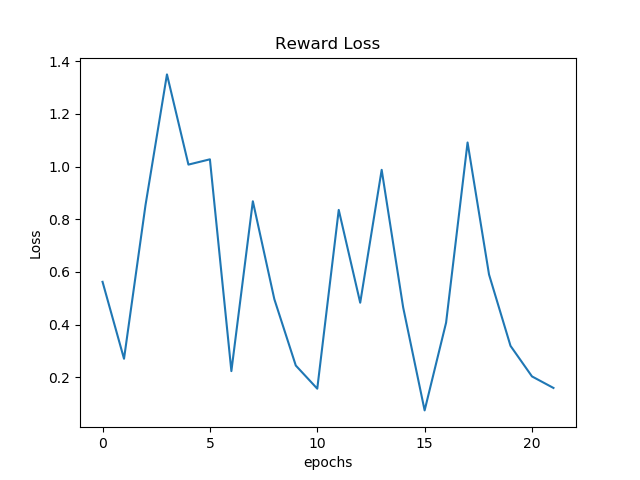
\includegraphics[width=0.45\linewidth]{data/reward_loss01.png} }%
	\subfloat{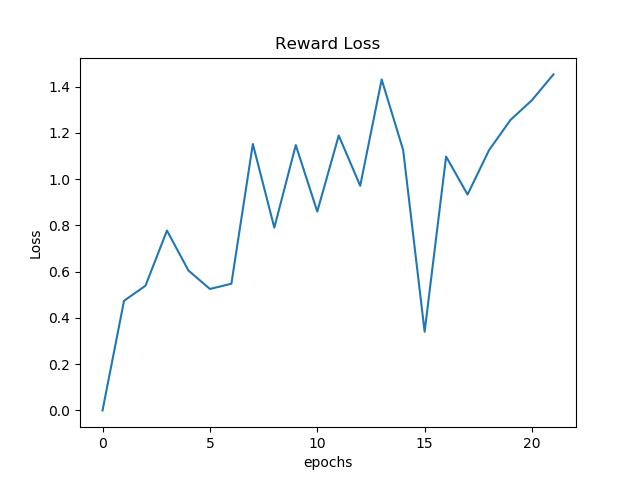
\includegraphics[width=0.45\linewidth]{data/reward_loss05.png} }%
	\caption{Comparison between loss of clips with label $(0,1)$ and $(1,0)$ (on the left) and indifferent labels (on the right).}
	\label{fig:loss0501}%
\end{figure*}
%%%%%%%%%%%%%%%%%%%%%%%%%%%%%%%%%%%%%%%%%%%%%%%%%%%%%%%%%%%%%%%%%%%%%%%%%%%%%%%%%%%%%%%%%%%%%%%

\subsection{Reward Model Loss}
In figure \ref{fig:rewardloss} is shown a particular effect which caught our attention, in essence that the reward loss rises with respect to the increase of the iterations number completed by the system. 
For better understanding this phenomenon we analyze the reward loss in two different components: one coming from all the clip labeled with $(0,1)$ and $(1,0)$; the other coming from the "indifferent labels", that are labeled with $(0.5,0.5)$. You can see the loss plot of the two components in Figure \ref{fig:loss0501}, the left one referred to images with label $(0,1)$ or $(1,0)$ and in the right one the "indifferent labels" loss.
These plots show the loss referred to a training process of 25 iterations for the reward model. 
%Here we split the reward loss in two different components: one coming from all the clip labeled with $(0,1)$ and $(1,0)$; the other coming from the "indifferent labels", that are labeled with $(0.5,0.5)$.
As we can observe from these plots, the losses from the $(0,1)$-$(1,0)$ preferences got a almost fixed range of values, $(0.2,1.4)$, while the ones computed from the "indifferent labels" yield increasing contributions to the overall reward model loss. 
This fact occurs for two main reasons: the number of the "indifferent labels" grows during the training process of the system and for reasons related to the definition of the reward loss function. 
The former is because, since the agent learns how to behave in the environment, after some epochs there are a lot of generated clips with agent steps in the right trajectory, that will be annotated with label $(0.5,0.5)$, so also the number of those "indifferent labels" in the annotation buffer will increase.
The latter comes directly from the definition of the reward loss function reported in section \ref{method} in equation \ref{eq:rewardloss}. The more the reward is accurate, the more $log(\hat{P}[\sigma^i \succ \sigma^j])$ will be close to $\mu(i)$, like every log-loss. When $\mu=(0,1)$ or $\mu=(1,0)$ one of the two terms of the sum will be 0 and the other very close to 1, in essence that will produce a loss almost 0. This does not happen if $\mu=(0.5,0.5)$, where both components of the loss function are non-zero and close to 0.5, which logarithm is not negligible value. For this reason computing the loss for pairs of clips with these labels will make the loss grown during the training protocol. 



\subsection{Resulting Configuration}

Our best configuration produces an agent that performs at every episode the "forced trajectory" both if we sampled actions from a Categorical distribution where logits are the output of the policy model, and if we use a greedy policy. Here the agent will compute always the action with the higher probability, that is an useful approximation when there is a higher action entropy. More in details we set the training protocol epochs to 80, the policy episodes to 150 and K to 1500; policy model has $0.0001$ of learning rate, while the reward model $0.0003$; the annotation are made by a sparse Oracle; after 25 epochs we stop the reward model training. This configuration is reported in Table \ref{table:config}. In Figure\ \ref{fig:rewardloss} and in Figure\ \ref{fig:losspolicy} we report the policy and the reward model loss of this configuration.

%%%%%%%%%%%%%%%%%%%%%%%%%%%%%%%%%%%%%%%%%%%%%%%%%%%%%%%%%%%%%%%%%%%%%%%%%%%%%%%%%%%%%%%%%%%%%%%
\begin{table}[h!]
    \centering
    \begin{tabular}{ |c|c|c|c| } 
        \hline
        \textbf{IRL Component} & \textbf{Parameter} & \textbf{Value} \\
          \hline
          \multirow{5}{*}{\textit{Policy}} & len episode & 150 \\ 
          & \# episodes & 150 \\ 
          & lr  & 0.0001 \\ 
          & std  & 0.5 \\
          & \# rewards & 300 \\
          \hline
          \multirow{2}{*}{\textit{Oracle}} & sparse & (-) \\ 
          & len clip & 5 \\
          \hline
          \multirow{3}{*}{\textit{Reward}} & K & 1500 \\ 
          & lr & 0.0003 \\ 
          & early stopping & 25 it. \\ 
          \hline
    \end{tabular}
    \label{table:config}
\end{table}
%%%%%%%%%%%%%%%%%%%%%%%%%%%%%%%%%%%%%%%%%%%%%%%%%%%%%%%%%%%%%%%%%%%%%%%%%%%%%%%%%%%%%%%%%%%%%%%

To test the reward model accuracy we used the reward model heat map, which is reported in Figure\ \ref{fig:heatmap}. The heat map represents the normalized rewards of all the possible states of the agent. In particular for each Minigrid cell, we take the maximum reward predicted by the reward model between the four possible orientations that the agent can assume and we normalize the resulting values. 
With this heat map we show how the reward model learns to assign higher rewards for those states in the "forced" direction, and lower ones to the other agent positions. The goal state has a small reward, that is because the reward model processes few goal state observations and because the agent episode ends immediately when he reaches this state. Another aspect to take in account is that the states in the fourth column of the heat map have a high reward, even if they do not correspond to the state of the forced trajectory. When the agent is facing up in one of the fourth column states, the Minigrid environment gives the same representation of that where the agent looks down in one of the first column states. For this reason, the reward model predicts similar reward for these symmetric states. 

